
\section{Мыцельскиан графа. Пример Зыкова–Мыцельского графа без треугольников со сколь угодно
большим хроматическим числом.}

\subsection{Мыцельскиан графа.}

Мыцельскиан графа $G$ -- граф $\mu(G) = (V', E'):$\\
$V = \{v_1, \dots, v_n, u_1, \dots, u_n, w\}$\\
$E' = E \cup \{(v_i, u_j)\, | \text{ если $(v_i, v_j) \in E$}\} \cup \{(w, u_i)\, | i = 1, \dots, n\}$\\
Пример: $G$ -- цикл длины 5 (черные ребра -- исходные):
\begin{center}
    \makebox[\textwidth][c]{\includegraphics[width=26cm, height=10cm]{mick.png}}
\end{center}

\subsection{Пример Зыкова–Мыцельского графа без треугольников со сколь угодно
большим хроматическим числом.}

Пусть $G_2 = K_2$, $G_3 = \mu(G_2), \dots, G_t = \mu(G_{t-1})$

Тогда $G_t$ -- граф без треугольников с $\rchi(G_t) = t$
{
    \color{gray}
\subsection*{\textit{Доказательство:}}
Полная индукция по $t$:

1) $G_t$ без треугольников:

Вершина $w$ не может быть в треугольнике, также не могут быть две вершины $u_i, u_j$ в треугольнике (по опр.). По предположению индукции треугольника $v_i, v_j, v_k$ тоже не может быть:

Пусть $v_i, v_j, u_k$ -- треугольник $\Rightarrow k \neq i, j$:
\[
\begin{cases}
    v_j \rightarrow u_k \Rightarrow \exists v_j \rightarrow v_k\\
    v_i \rightarrow u_k \Rightarrow \exists v_i \rightarrow v_k
\end{cases}
\Rightarrow
\text{ есть треугольник $v_i, v_j, v_k \Rightarrow$ противоречие}
\]
\\
2) a) $\rchi(G_t) \leq t$:

$\rchi(G_{t-1}) = t - 1$. Красим $u_i$ в цвет $v_i$. $w$ красим в новый цвет $\Rightarrow$ покрасили в $t$ цветов.
\\\\
б)$\rchi(G_t) \geq t$:

От противного: $\rchi(G_t) = t-1$:

Пусть раскрасили в $t-1$ цвет и $w$ имеет цвет $t-1$. Тогда $u_i$ раскрашены в цвета $(1, \hdots, t-2)$. Перекрашиваем $v_i$:
\[
\text{цвет }v_i = \begin{cases}
    \text{прежний, если он не $t-1$}\\
    \text{цвет $u_i$, если он $t-1$}
\end{cases}
\]
Вершины $v_i$ цвета $t-1$ найдутся по предположению индукции.

Тем самым $G_{t-1}$ раскрашен в $t-2$ цвета и для подграфа $G_{t-1}$ раскраска правильная:

(Иначе были $v_i \leftrightarrow v_j$ с одинаковым цветом $x$, поменяли цвет одной из вершин $\Rightarrow$ раньше в $v_i$ был цвет $t-1$ но поменяли на цвет $x$ который у $u_i$. Между $u_i$ и $v_j$ есть ребро $\Rightarrow$ противоречие (они одного цвета до изменений цветов))

Получается мы раскрасили $G_{t-1}$ в $t-2$ цвета $\Rightarrow$ противоречие
}

\section{Паросочетания и вершинные покрытия в графе. Утверждение о связи максимального размера
паросочетания и минимального размера вершинного покрытия в произвольном графе. Теорема
Кёнига.}

Паросочетание в $G$ -- $M \subseteq E: \forall m_1, m_2 \in E: m_1 \cap m_2 = \emptyset$

Вершинное покрытие в $G$ -- $U \subseteq V: \forall \{a, b\} \in E: (a \in U) \lor (b \in U)$

В произвольном графе:
\[
|M_{max}| \leq |U_{min}|
\]
Если достигается равенство $\Leftrightarrow \exists$ парсоч. и мин. покр равного размера
\vspace{-2cm}
{
        \color{gray}
\subsection*{\textit{Доказательство:}}
Пусть $M'$ -- парсоч, $U'$ -- вершин. покрытие и $|M'| = |U'|$:
\[
|M'| \leq |M_{max}| \leq |U_{min}| \leq |U'|
\]
\[
\Downarrow
\]
\[
|M_{max}| = |U_{min}|
\]
}


Чтобы покрыть все ребра из $M$ нужно как минимум $|M|$ вершин
\subsection{Теорема Кёнига}
В двудольном графе $G$ выполняется равенство:
\[
|M_{max}| = |U_{min}|
\]

\section{Чередующийся и увеличивающий пути относительно паросочетания в двудольном графе.}

Пусть $G = (L \cup R, E)$ -- двудольный граф и $M$ -- паросочетание. 

Чередующийся путь относительно $M$ -- путь (без повторений по ребрам), начинающийся в $a \in L$ не покрытой $M$ и в котором ребра чередуются по принадлежности $M$

Увеличивающий путь относительно $M$ -- чередующийся путь из $a$ в $b$: $b$ тоже не покрыта $M$

\begin{center}
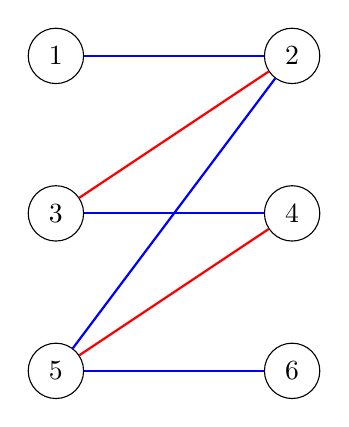
\begin{tikzpicture}[
    % Стиль для вершин: круг, нарисовать границу, белый фон
    vertex/.style={circle, draw, fill=white, minimum size=20pt, inner sep=0pt},
    % Стиль для ребер: толстая линия
    edge/.style={thick}
]

    % --- Вершины левой доли (1, 3, 5) ---
    % Располагаем их вертикально (координата Y меняется: 4, 2, 0)
    \node[vertex] (v1) at (0, 4) {1};
    \node[vertex] (v3) at (0, 2) {3};
    \node[vertex] (v5) at (0, 0) {5};

    % --- Вершины правой доли (2, 4, 6) ---
    % Сдвигаем вправо (X=3) и выравниваем по тем же высотам
    \node[vertex] (v2) at (3, 4) {2};
    \node[vertex] (v4) at (3, 2) {4};
    \node[vertex] (v6) at (3, 0) {6};

    % --- Красные ребра (3-2, 5-4) ---
    \draw[edge, red] (v3) -- (v2);
    \draw[edge, red] (v5) -- (v4);

    % --- Синие ребра (1-2, 3-4, 5-6) ---
    \draw[edge, blue] (v1) -- (v2);
    \draw[edge, blue] (v2) -- (v5);
    \draw[edge, blue] (v3) -- (v4);
    \draw[edge, blue] (v5) -- (v6);

    % --- Подписи долей (опционально) ---
    %\node at (0, -1) {Левая доля};
    %\node at (3, -1) {Правая доля};

\end{tikzpicture}
\\
1-2-3-4 -- чередующийся путь\\
1-2-3-4-5-6 -- увеличивающийся путь
\end{center}

Если относительно $M$ есть увеличивающийся путь $\Rightarrow$ $M$ -- не максимальное паросочетание

\section{Условие Холла для двудольного графа, теорема Холла}
\subsection{Теорема Холла}

В двудольном графе $G = (L \cup R, E)$:
\begin{center}
    $\exists$ паросочетание размера $|L| \Leftrightarrow \underbrace{\forall S \subseteq L: |N(S)| \geq |S|}_{\text{условие Холла}}$
\end{center}

Для $S \subseteq L: N(S) = \{y \in R \; | \; \exists x \in S: \{x, y\} \in E\}$

{
    \color{gray}
\subsection*{\textit{Доказательство:}}
}

\section{Клика и независимое множество в графе. Теорема Рамсея. Верхняя оценка чисел Рамсея}

Размер наибольшей клики в $G$ -- $\omega(G)$

Размер наибольшего нез. мн-ва в $G$ -- $\alpha(G)$

Пусть $n ,k \geq 1: R(n,k)$ -- наименьшее $N$ такое, что $\forall G$ на $N$ вершинах найдется либо клика размером $k$, либо нез. мн-во размера $n$

Свойства:
\begin{itemize}
    \item $R(n,k) = R(k, n)$ (дополнение $\overline{G}$)
    \item $R(1,k) = 1$
    \item $R(2, k) = k$
\end{itemize}

\subsection{Теорема Рамсея}
$\forall n, k \geq 2: R(n,k)$ -- конечно
\[
R(n,k) \leq R(n-1, k) + R(n, k - 1)
\]
Верхняя оценка:
\[
R(n,k) \leq \binom{n+k-2}{n-1} = \binom{n+k-2}{k-1}
\]

\section{Частично упорядоченные множества: строгий и нестрогий частичные порядки, линейный порядок. Утверждение о связи строгого и нестрогого порядков.}

Пусть $A \neq \emptyset$ -- мн-во:

Отношение $R$ на $A$ является отношением $\textbf{строгого}$ частичного порядка, если:
\begin{enumerate}
    \item $\lnot aRa$ -- Иррефлексивность
    \item $aRb \land bRc \Rightarrow aRc$ -- Транзитивность
\end{enumerate}
\text{}
\\
Отношение $R$ на $A$ является отношением $\textbf{нестрогого}$ частичного порядка, если:
\begin{enumerate}
    \item $aRa$ -- Рефлексивность
    \item $aRb \land bRa \Rightarrow a = b$ -- Антисимметричность
    \item $aRb \land bRc \Rightarrow aRc$ -- Транзитивность
\end{enumerate}
\text{}
\\
Линейный порядок -- частичный порядок, в котором любые два элемента сравнимы

\subsection{Связь строгого и нестрогого порядков}

Из строгого порядка можно получить нестрогий и наоборот:
\begin{enumerate}
    \item Пусть $\leq$ -- нестрогий порядок. Тогда
    \[
    < \; := \; \leq \setminus \; \{(a,a) \; | \; a \in A\}
    \]
    \item Пусть $<$ -- строгий порядок. Тогда
    \[
    \leq \; := \; < \cup \; \{(a,a) \; | \; a \in A\}
    \]
\end{enumerate}

\section{Операции с частично упорядоченными множествами: сумма порядков, покоординатный порядок,
лексикографический порядок.}

Частично упорядоченное множество (ЧУМ) -- мн-во с заданным отн. порядка: $(A, <)$ или $(A, \leq)$

Пример:
\begin{enumerate}
    \item $(\mathbb{N}, \, \mid) \; a \leq b \Leftrightarrow a \mid b$
    \item $(\mathbb{Z}, \, \mid)$ -- не ЧУМ $(-1 \mid 1) \land (1 \mid -1) \not \Rightarrow 1 = -1$
    \item $(2^A, \subseteq)$ -- ЧУМ
\end{enumerate}

\subsection{Операции с ЧУМ}
\begin{enumerate}
    \item Сумма порядков:\\{
        Пусть $(A, \leq_{A})$, $(B, \leq_{B})$ -- ЧУМ. Сумма $A+B$ -- $A \sqcup B$:
        \begin{itemize}
            \item Внутри $A$ порядок $\leq_{A}$
            \item Внутри $B$ порядок $\leq_{B}$
            \item Все элементы из $A$ меньше всех элементов из $B$
        \end{itemize}
    }
    \item Покоординатный порядок:{
        \[
        (A \times B, \leq): (a_1, b_1) \leq (a_2, b_2) \Leftrightarrow \begin{cases}
            a_1 \leq_{A} a_2\\
            b_1 \leq_{B} b_2
        \end{cases}
        \]
    }
    \item Лексикографический порядок:{
        \[
        (A \times B, <): (a_1, b_1) < (a_2, b_2) \Leftrightarrow a_1 <_{A} a_2 \; \lor \begin{cases}
            a_1 = a_2\\
            b_1 <_{B} b_2
        \end{cases} 
        \]
    }
\end{enumerate}

\section{Минимальные и максимальные элементы в частичных порядках. Наибольшие и наименьшие элементы. Их свойства. Примеры порядков: с бесконечным числом минимальных элементов, с единственным минимальным элементом, но не наименьшим.}

Пусть $(P, \leq_{P})$ -- ЧУМ:
\[
\begin{cases}
    a \in P \text{ -- минимальный, если $\not \exists b \in P: b < a$}\\
    a \in P \text{ -- наименьший, если $\forall b \in P: a \leq b$}\\
    a \in P \text{ -- максимальный, если $\not \exists b \in P: b > a$}\\
    a \in P \text{ -- наибольший, если $\forall b \in P: a \geq b$}\\
\end{cases}
\]
Наименьший/наибольший -- единственный, если существует

Наименьший/наибольший является минимальным/максимальным

Примеры:
\begin{itemize}
    \item $(\mathbb{Z} \cup \{*\}, \; \leq \; )$: минимальный -- $*$, наименьшего -- нет
    \item $([0,1]^2, \leq)$ -- покоординатный:\\{
        \begin{tikzpicture}[scale=0.8,>=Latex]
        % background grid
        \draw[step=0.5, very thin, gray!25] (-3,-2) grid (4,4);

        % axes
        \draw[thick,->] (-3,0) -- (4,0);
        \draw[thick,->] (0,-2) -- (0,4);

        % curve (hand-drawn style shape similar to your sketch)
        \draw (0,0) rectangle (2,2);
        \fill[gray!30] (0,0) rectangle (2,2);
        % red point near origin
        \fill[red] (0,0) circle (2.5pt);

        % red arrow + label "наш"
        \draw[red,thick,->] (1.6,-1.1) -- (0.15,-0.05);
        \node[red] at (1.95,-1.15) { наим. и мин.};
        \end{tikzpicture}
    }
    \item $(\{|x|+|y| = 1\}, \leq)$ -- покоординатный:\\{
        \begin{tikzpicture}[scale=0.8,>=Latex]

  % grid
  \draw[step=0.5, very thin, gray!25] (-4,-3) grid (6,4);

  % axes
  \draw[thick,->] (-4,0) -- (6,0);
  \draw[thick,->] (0,-3) -- (0,4);

  % diamond |x|+|y|=1 with vertices (±1,0),(0,±1)
  \draw[thick] (0,1) -- (1,0) -- (0,-1) -- (-1,0) -- cycle;

  % highlight the "lower" side segment in red (between (-1,0) and (0,-1))
  \draw[red, line width=3.2pt, line cap=round] (-1,0) -- (0,-1);

  % optional point at top vertex (as in sketch)
  \fill (0,1) circle (1.3pt);

  % red arrow + label "наш"
  \draw[red,thick,->] (2.2,-2.0) -- (0.1,-0.9);
  \node[red] at (2.45,-2.05) {\small минимальные};

  % red note "нет наши"
  \node[red] at (4.3,-2.6) {\small нет наименьших};

\end{tikzpicture}
    }
\end{itemize}

\section{Изоморфизм порядков, примеры. Отрезки в частично упорядоченных множествах, их образы при
изоморфизме. Теорема об изоморфизме счётных плотных линейных порядков без наименьшего и
наибольшего элемента}

\subsection{Изоморфизм порядков, примеры}
Пусть $(P, \leq_{P})$, $(Q, \leq_{Q})$ -- ЧУМ. $P \simeq Q$, если $\exists$ биекция $h: P \rightarrow Q$:
\[
\forall x, y \in P: x \leq_{P} y \Leftrightarrow h(x) \leq_{Q} h(y)
\]
Примеры:
\begin{itemize}
    \item $(\mathbb{N}, \leq) \simeq (\{2, 4, 6, \hdots\}, \leq)$ -- биекция $f(n) = 2n$
    \item $(\mathbb{Q}, \leq) \not \simeq (\mathbb{R}, \leq)$ -- нет биекции между $\mathbb{Q}$ и $\mathbb{R}$
\end{itemize}

Инварианты:
\begin{itemize}
    \item Мощность (из счетного нет биекции в континуум и т.д.)
    \item $(\mathbb{Q}, \leq) \not \simeq (\mathbb{Z}, \leq)$ -- $\mathbb{Q}$ -- плотный, $\mathbb{Z}$ -- нет
    \item $([0, 1], \leq) \not \simeq ((0,1), \leq)$ -- в интервале нет наименьшего/наибольшего
    \item Наличие непосредственных предшественников/последователей
\end{itemize}

\subsection{Отрезки в частично упорядоченных множествах, их образы при
изоморфизме}

Если $\varphi: P \rightarrow Q$ -- изоморфизм $P, Q \Rightarrow \varphi([a, b]) = [\varphi(a), \varphi(b)]$

\subsection{Теорема об изоморфизме счётных плотных линейных порядков без наименьшего и
наибольшего элемента}

Плотный порядок: $\forall a < b: \exists c: a < c < b$

Теорема: Любые два счётных плотных линейных порядка без наим/наиб элемента изоморфны

\section{Бесконечно убывающие цепи. Принцип математической индукции для частично упорядоченных
множеств. Фундированные множества, теорема об эквивалентности трех определений фундированного множества.}

Бесконечно убывающая цепь в ЧУМ $(A, <)$ -- последовательность:
\[
a_1 > a_2 > a_3 > \hdots
\]

\subsection{Фундированные множества, теорема об эквивалентности трех определений фундированного множества.}

Для ЧУМ $(P, \leq)$ следующие определения эквивалентны:
\begin{enumerate}
    \item $P$ -- фундированное $(\forall S \subseteq P: \exists \, min(S))$
    \item $\not \exists$ бесконечно убывающих цепей
    \item Для $P$ справедлив принцип индукции:\\{
        Для $\forall$ семейства подмножеств:
        \[
        \{A(p) \; | \; p \in P\}
        \]
        \[
        \forall p \in P \; (\forall q < p: A(q) = 1) \Rightarrow A(p) = 1
        \]
    }
\end{enumerate}
База индукции -- проверить утверждения на минимальных элементах
